\documentclass{pginz}

%%%%%%%%%Miejsce na dodatkowe pakiety%%%%%%%%%%%%%
\usepackage{subcaption}

\begin{document}

\chapter*{Introduction}

The project described in this documentation consisted of developing an Instance Segmentation software using the image captured by an Intel RealSense D435 camera. It was realised in the summer semester of the 2022/23 academic year as part of the subject "Integrated decisive systems" (pl. \textit{Zintegrowane systemy decyzyjne}).

\noindent The project team consisted of:
\begin{itemize}[noitemsep,topsep=0pt,parsep=0pt,partopsep=0pt]
    \item Jakub Pilarski - leader
    \item Weronika Kapusta - vice-leader
    \item Andrzejewski Miłosz
    \item Iskrzycki Paweł
    \item Kołoszko Mateusz 
    \item Koncewicz Gabriela
    \item Szymanek Tomasz
    \item Urbański Filip 
\end{itemize}

The task required us to devise a method of Instance Segmentation. Afterwards, the shape of the object had to be determined based on the voxels belonging to it (by using e.g. a 3D bounding box). It was also necessary to devise our own dataset for model training.

\noindent Our initial project assumptions were as following:
\begin{itemize}[noitemsep,topsep=0pt]
    \item real-time work using RGBD RealSense D435 camera;
    \item static objects detection;
    \item object size limited from 0.1[m]x0.01[m]x0.01[m] to 1[m]x1[m]x1[m]
    \item final accuracy
    \begin{itemize}[noitemsep,topsep=0pt]
        \item segmentation accuracy > 80\%
        \item IoU > 60\%
    \end{itemize}
\end{itemize}

The following document serves as a proof of our work during the semester as well as an explanation on the program's operating principles and user manual. The GitLab repository containing the project's source code can be found \href{https://git.pg.edu.pl/p1304095/zsd-is}{\textit{here}}.


\tableofcontents
\addcontentsline{toc}{chapter}{Contents}

% wprowadzenie (1 str),                     OK
% przegląd podobnych rozwiązań (2 str),     OK
% opis własnego rozwiązania (2 str),        OK
% wyniki testów (2 str.),                   OK
% podsumowanie (1 str),                     OK
% dalsze możliwości (1 str.),               OK
% napotkane problemy i rozwiązania (...)    OK
% bibliografia (ok 30 pozycji).             OK
% Wartości w nawiasach są orientacyjne (raczej minimalne).


\chapter{Review of existing solutions}
Image Segmentation is not a new concept and is widely used in various areas such as machine vision. It is also a topic of many research papers and coding projects. While conducting research for our project, we encountered many different similar solutions both in terms of overall instance segmentation as well as essential parts of our project, like dataset preparation or raw image, point cloud and stream filtration. This chapter covers some of the solutions that we either took inspiration from or that helped us understand crucial concepts.


%=======================================
\section{DETR}
DETR \cite{carion2020endtoend} (DEtection TRansformer) approaches object detection as a direct set prediction problem. It consists of a set-based global loss, which forces unique predictions via bipartite matching, and a Transformer encoder-decoder architecture. Given a fixed small set of learned object queries, DETR reasons about the relations of the objects and the global image context to directly output the final set of predictions in parallel. Due to this parallel nature, DETR is very fast and efficient.

\begin{figure}[ht]
    \centering
    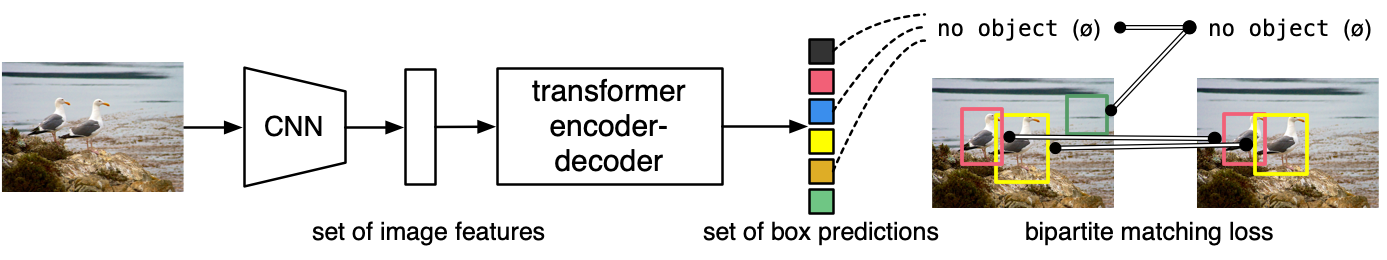
\includegraphics[width=1.0\textwidth]{img/DETR.png}
    \caption{DETR's architecture as presented in the paper \cite{carion2020endtoend}.}
    \label{fig:detr-architecture}
\end{figure}


In the first stage (\cref{fig:detr-architecture}), feature maps are extracted from the images via a Backbone layer. Many different models can be used, such as RestNet-50 or ResNet-101 \cite{he2015deep}. In this way, 2-dimensional structure information is preserved. In the following stages, the data is flattened, so we get a 1-dimensional structure. After positional encoding, it is transferred to the encoder-decoder mechanism. Finally, each output is forwarded to the Feed Forward Network.

The last layer consists of 3 nodes. The normalized center coordinates of the predicted object and the predicted height and width values of the object are obtained where the Relu activation function is used. The class of the relevant object is predicted where the softmax activation function is used in the node. Thus, there is no need for Non-Maximum Suppression (NMS).

In the Positional Encoding section, the vector of each element (or token in NLP world) is re-created according to its place in the array. Thus, the same word can have different vectors at different positions in the array.
In the encoder layer, the reduction of high-dimensional feature matrix to lower-dimensional feature matrices is performed. It consists of multi-head self attention, normalizer and feed forward network modules in each encoder layer.
In the decoder layer, there are multi-head self attention, normalizer and feed forward network modules just like the encoder. N number of object queries are converted as output embedding. In the next stage, final estimation processes are carried out with the feed forward network.



%=======================================
\section{OneFormer}
OneFormer \cite{jain2023oneformer} is a universal image segmentation framework jointly trained on the panoptic, semantic, and instance segmentation. It outperforms existing state-of-the-arts on all three image segmentation tasks, by only training once on one panoptic dataset, instead of having to be trained separately for each task. Since 2023, it is available as a part of HuggingFace's \textit{transformers} \cite{huggingface-transformers} library.

\begin{figure}[ht]
    \centering
    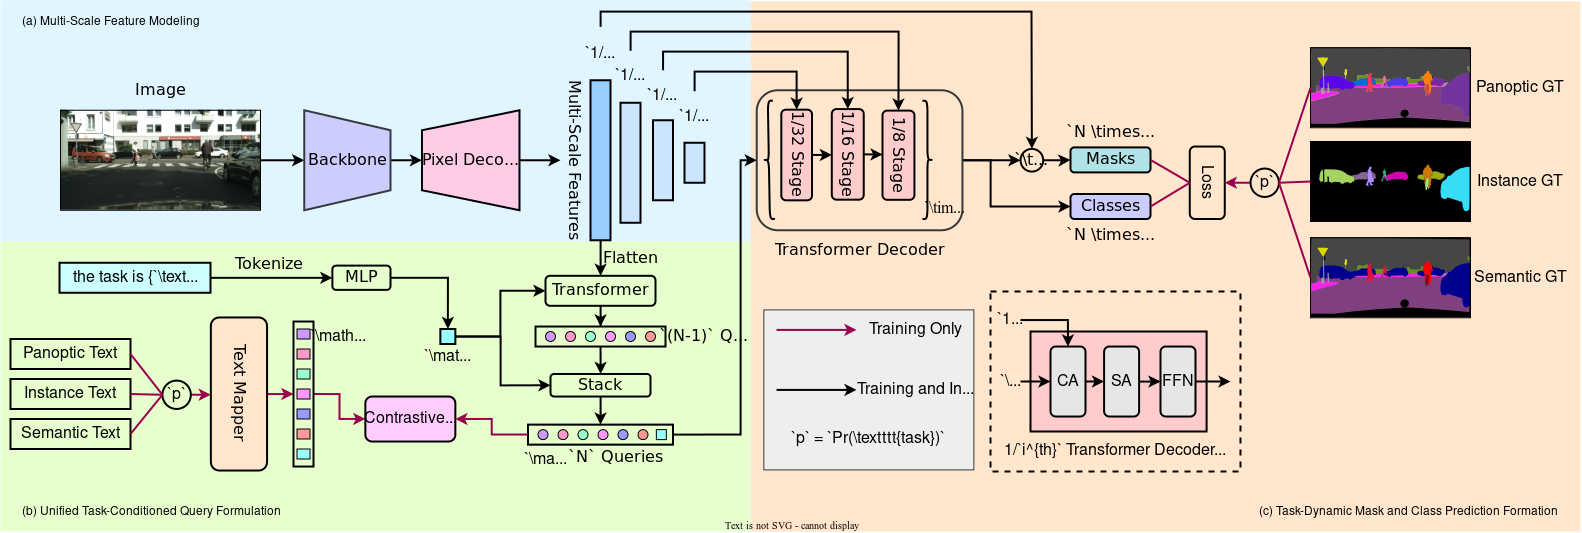
\includegraphics[width=1.0\textwidth]{img/oneformer.png}
    \caption{OneFormer's framework as presented in the paper \cite{jain2023oneformer}. The framework was implemented using Detectron2 \cite{wu2019detectron2} library. }
    \label{fig:oneformer-framework}
\end{figure}


The authors prepared a large number of pre-trained models with different backbones as well as trained and validated on different datasets, all of which can be downloaded from the project's github repository \cite{oneformer-repo}:
 
\begin{itemize}
    \item Backbones - the available models utilise commonly used backbones pretrained on the ImageNet-22K \cite{deng2009imagenet} to extract multi-scale feature representations from the input image. Then, a pixel decoder with a \textit{Multi-Scale Deformable Transformer} \cite{zhu2020deformable, cheng2021mask2former} based architecture aids the feature modeling by gradually upsampling the backbone features. The Swin-Transformer \cite{liu2021Swin}, ConvNeXt \cite{liu2022convnet}, and DiNAT \cite{hassani2022dilated} backbones were used for the experiments.
    \item Datasets - the models were trained with a batch size of 16, on three popular datasets that support the three aforementioned segmentation tasks: semantic, instance and panoptic. The datasets used are ADE20K \cite{zhou2019semantic, zhou2017scene}, CityScapes \cite{Cordts2016Cityscapes}, and COCO \cite{lin2015microsoft}.
\end{itemize}


%=======================================
\section{ISBNet}
ISBnet \cite{ngo2023isbnet} is a neural network model developed by VinAI Research, designed to tackle the task of instance segmentation, which involves identifying and delineating specific objects within an image. It leverages advanced deep learning techniques to accurately and efficiently segment objects, making it a valuable tool for computer vision applications.
To address the limitations of DyCo3D \cite{He2021dyco3d}, researchers proposed ISBNet, a cluster-free framework for 3DIS with Instance-aware Farthest Point Sampling and Box-aware Dynamic Convolution.

An auxiliary branch of the model jointly predicts the axis-aligned bounding box and the binary mask of each instance. The ground-truth axis-aligned bounding box is deduced from the existing instance mask label.

\begin{figure}[ht]
    \centering
    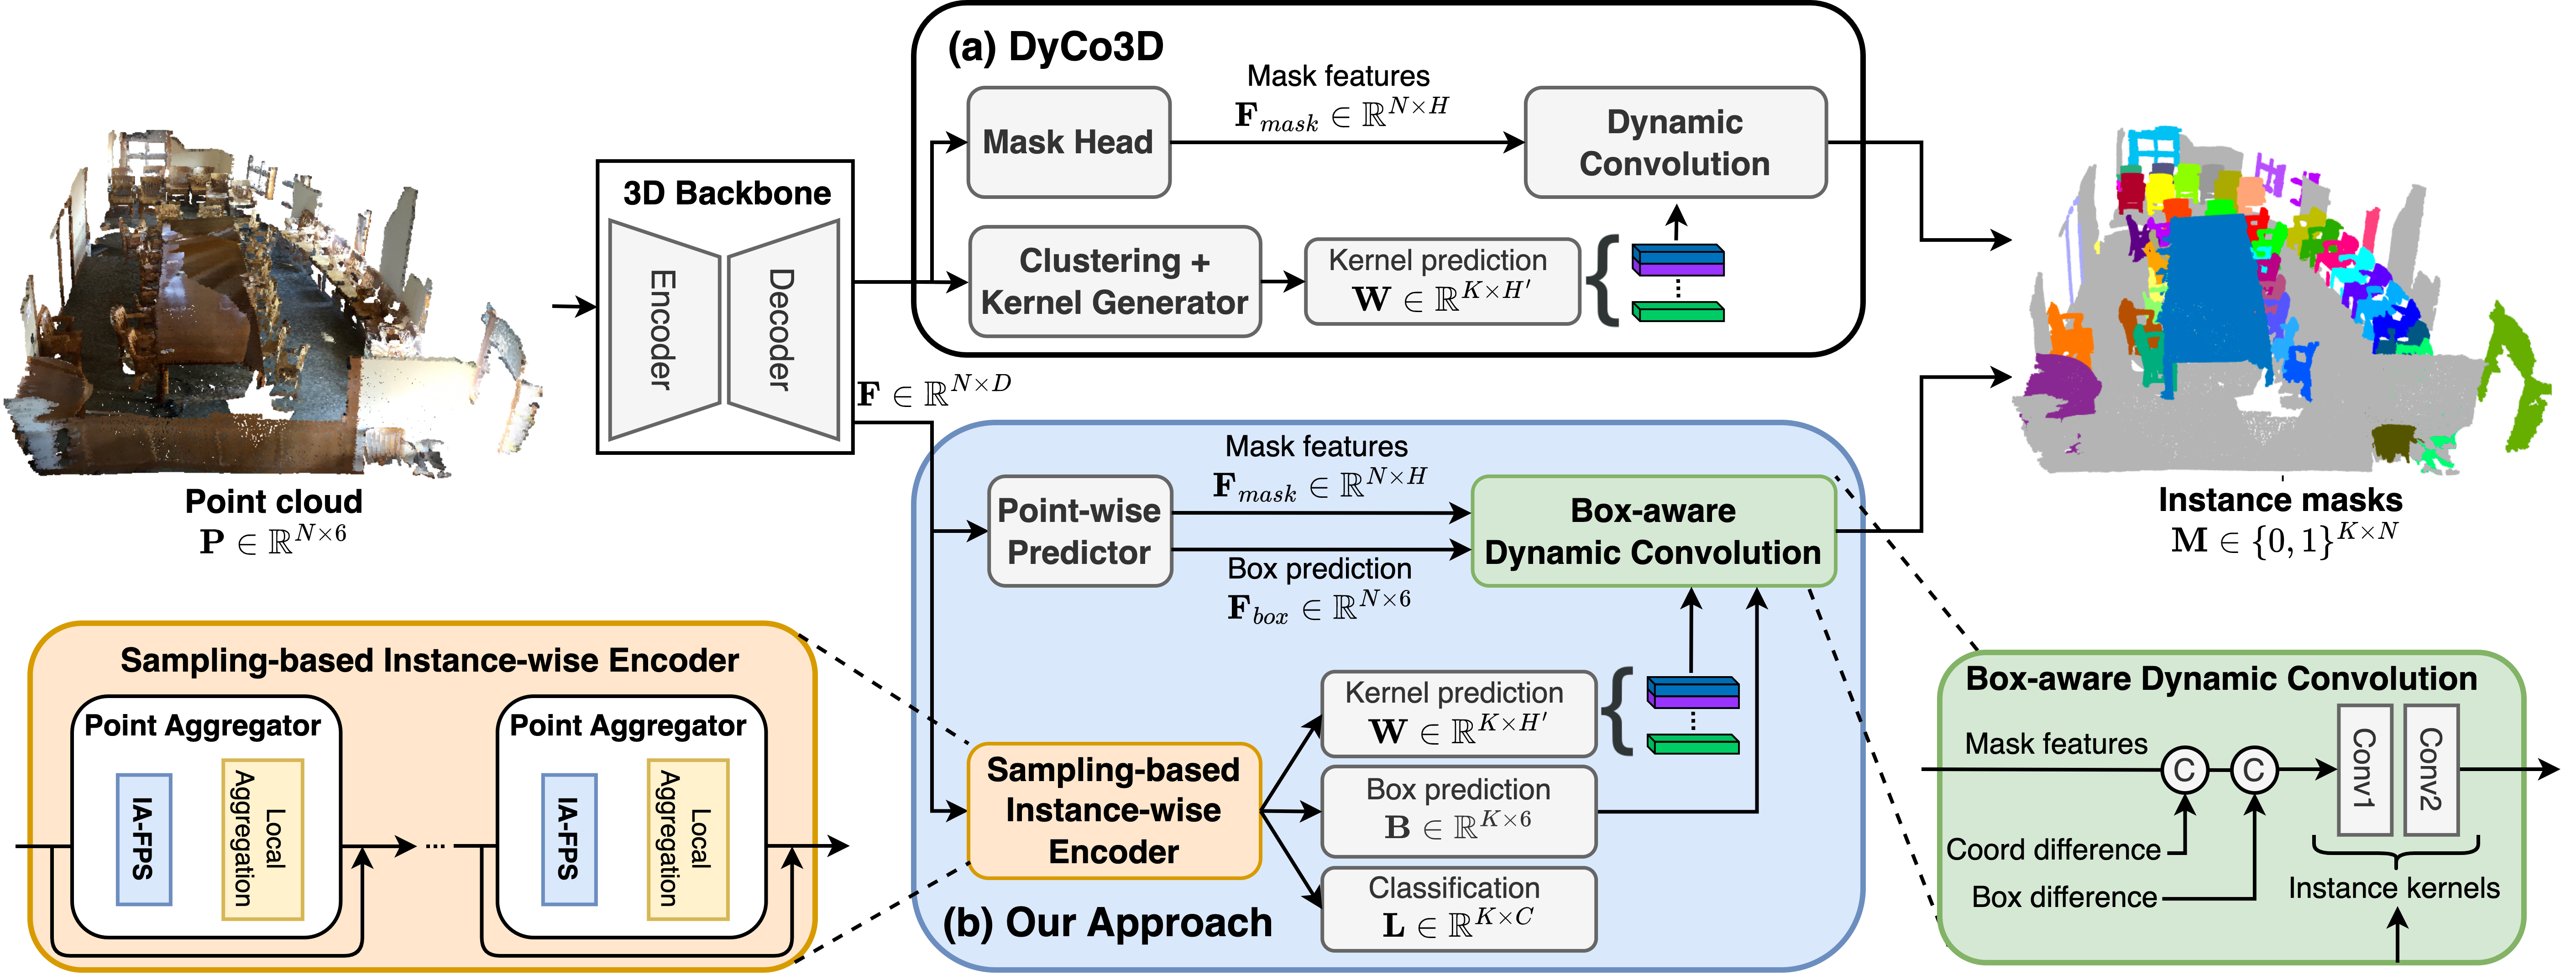
\includegraphics[width=1.0\textwidth]{img/isbnet_arch.png}
    \caption{Architectures of DyCo3D (block a) and ISBNet's approach (block b), as presented in the paper \cite{ngo2023isbnet}.}
    \label{fig:isbnet-architecture}
\end{figure}
	
Given a point cloud, a 3D backbone is employed to extract per-point features (\cref{fig:isbnet-architecture}). For DyCo3D, it first groups points into clusters based on the predicted object centroid from each point to generate a kernel for each cluster. In the meantime, the mask head transforms the per-point features into mask features for dynamic convolution. In ISBNet, the clustering algorithm is replaced with a novel sampling-based instance-wise encoder to obtain faster and more robust kernel, box, and class predictions. Furthermore, a point-wise predictor replaces the mask head of DyCo3D to output the mask and box features for a new box-aware dynamic convolution to produce more accurate instance masks.

ISBNet not only achieves the highest accuracy among these three datasets, surpassing the strongest method by +2.7/2.4/3.0 on Scan-NetV2 \cite{dai2017scannet}, S3DIS \cite{armeni2017joint}, and STPLS3D \cite{Chen_2022_BMVC}, but also demonstrates to be highly efficient, running at 237ms per scene on ScanNetV2.



%=======================================
\section{Amodal3Det}
Amodal3Det \cite{zhuo17amodal3det} is a neural network model available on GitHub and developed by the Phoenix Neural Networks team. It focuses on the challenging task of amodal 3D object detection, which involves detecting and localizing objects in 3D space, even when they are partially occluded or invisible. This model incorporates state-of-the-art techniques in deep learning and computer vision to address the complex problem of accurately detecting objects in challenging scenarios. The architecture of the Amodal3Det network is based on state-of-the-art techniques in deep learning and computer vision. 

\begin{figure}[ht]
    \centering
    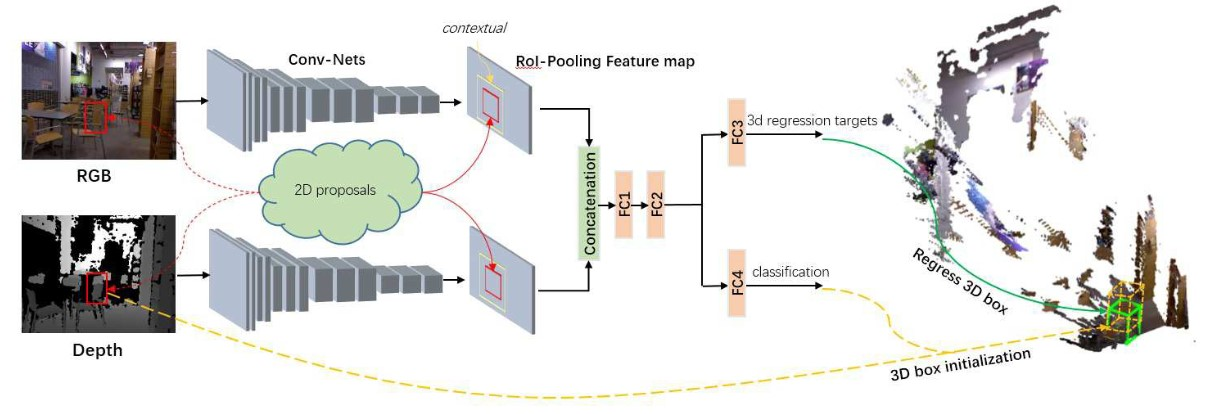
\includegraphics[width=1.0\textwidth]{img/amodal3det.jpg}
    \caption{Overview of Amodal3Det's 3D object detection system. For each 2D segment proposal, firstly the localization of a 3D box is initialized (yellow dash box) based on depth information and its size according to class wise prior knowledge. Then object class and 3D regression offsets are jointly learned based on 2D features only, with the goal of obtaining the final 3D detection (green solid box) by adjusting the location, dimension, and orientation of the initial 3D box.}
    \label{fig:amodal-arch}
\end{figure}


The labeled NYU Depth V2 \cite{Silberman:ECCV12} dataset is one of the most popular but very challenging dataset in the RGBD scene understanding research community. The original version provides 1449 RGB-Depth indoor scene images with dense 2D pixel wise class labels. To enrich the labeling features and encourage 3D object detection research, in the SUN RGBD dataset \cite{sunrgbd} (superset of NYUV2) researchers added extra 3D bounding boxes and room layouts to ground truth annotations. Since depth maps are imperfect in reality due to measurement noise, light reflection and absorption, and occlusion etc, they also refined the quality of depth maps by integrating multiple RGB-D frames from the NYUV2 raw video data.

Given a pair of color and depth images, the goal of the amodal 3D object detection is to identify the object instance locations and its full extent in 3D space. Objects that were used were a bathtub, bed, bookshelf, box, chair, counter, desk, door, dresser, garbage bin, lamp, monitor, nightstand, pillow, sink, sofa, table, tv, toilet. 

To train the Amodal3Det model, the Phoenix Neural Networks team utilized large-scale datasets specifically curated for amodal 3D object detection. These datasets would consist of 3D scenes with various objects in different poses, occlusion levels, and viewpoints. The annotations in the training data would include the 3D bounding box information for both visible and occluded parts of the objects, providing the model with the necessary supervision to learn the task effectively.



%=======================================
\section{DeepLabV3}
DeepLabV3 \cite{deeplabv3plus2018, chen2017rethinking} is a state-of-the-art deep learning model designed for semantic image segmentation. The underlying architecture of DeepLabV3 is based on a convolutional neural network (CNN) framework. The model consists of an encoder network, which extracts high-level features from the input image, and a decoder network, which generates dense pixel-level predictions.

The DeepLabV3 model takes an image as input. Following this action the input image is fed into a pre-trained CNN, such as ResNet \cite{he2015deep} or MobileNet \cite{mobilenetv32019}, which acts as the encoder network. Atrous Convolutions (dilated convolutions) are applied which increase the receptive field without reducing the spatial resolution. This allows the model to capture both local and global contextual information effectively. Next the Atrous Spatial Pyramid Pooling (ASPP) is used which involves applying atrous convolutions with different dilation rates in parallel to capture context at multiple scales. This enables the model to incorporate both fine-grained details and global context into its predictions. Then the decoder employs bilinear upsampling to increase the spatial resolution of the feature maps. Using skip connections, high-resolution future maps are combined from the encoder network with upsampled feature maps from the decoder network. This helps to preserve local information and enhance the segmentation accuracy. Finally the combined feature maps are further processed through additional convolutional layers to generate the final dense pixel-wise predictions. The output is a segmentation map, where each pixel is assigned a label corresponding to a specific object class. 

While working with DeepLabV3 we decided to create our own dataset based on the ADE20K \cite{zhou2017scene, zhou2019semantic}, which would include objects photographed in the laboratory.


\chapter{Solution Overview}
Our work on the project could be divided into 4 different aspects we focused on. The task required us to create our own dataset for neural network training, as well as to devise an algorithm calculating objects' bounding boxes. The program had to be then connected to the RGBD cameras and made into a user-friendly application. The following flowchart illustrates the working principle of the program:

\begin{figure}[ht]
    \centering
    \includesvg[scale=0.4]{img/app-flowchart.svg}
    \caption{Flowchart showing the program's operating principle.}
    \label{fig:app-flowchart}
\end{figure}

\section{Dataset preparation}
After considering the size of the photo box and the availability of certain everyday objects, we chose 7 different classes:
\begin{itemize}[noitemsep,topsep=0pt,parsep=0pt,partopsep=0pt]
    \item mug
    \item box
    \item wine glass
    \item bowl
    \item shoe
    \item cap
    \item lamp
\end{itemize}
Our initial plans were to also include a \textit{bottle} class, however after encountering several problems, mainly concerning the way the light rays passed through the bottles, we were forced to narrow it down.

\subsection{Obtaining photo data}
To obtain RGB and depth image data we used Intel's \textit{RealSense Viewer} application, which is a part of Intel® RealSense™ SDK 2.0 \cite{realsense-sdk}. We recorded short sequences and saved them as .bag files, from which we later extracted the RGB image and depth data in form of a point cloud.

\begin{figure}[ht]
    \centering
    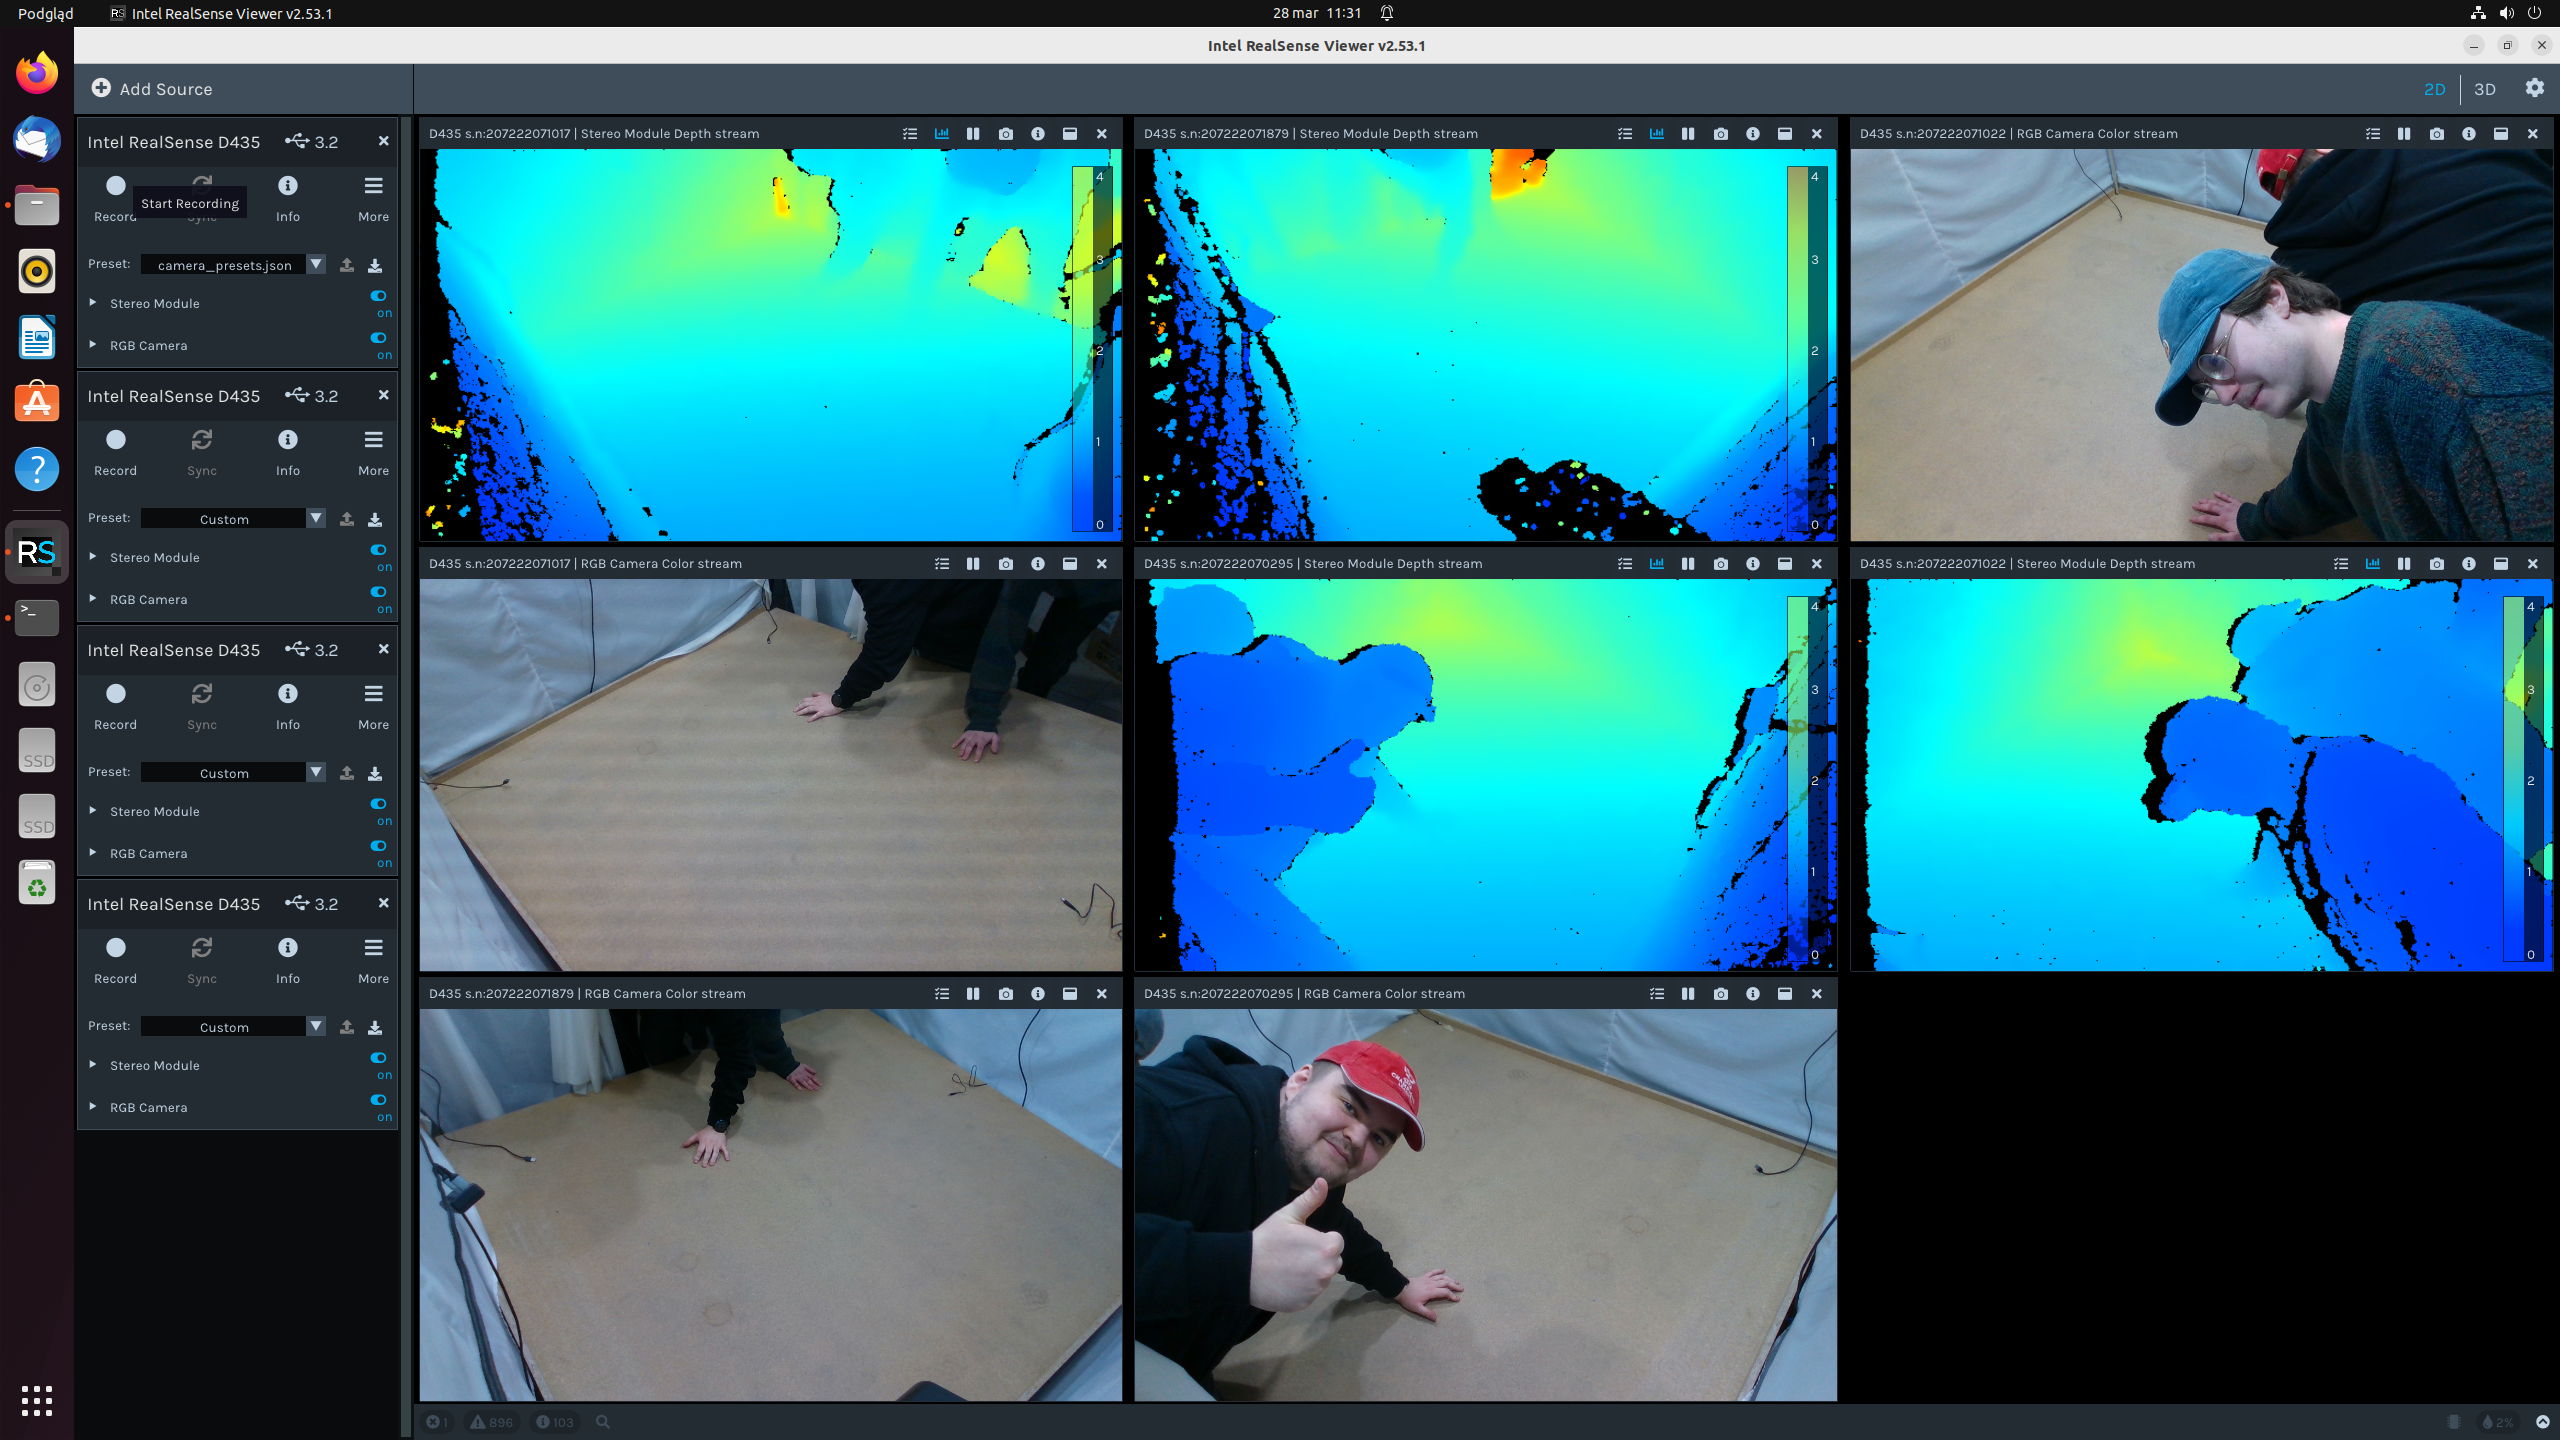
\includegraphics[width=0.75\textwidth]{img/viewer-screenshot.png}
    \caption{Intel's RealSense Viewer window showing capturing data from the cameras.}
    \label{fig:realsense-viewer}
\end{figure}

Preparing the data in the lab took about 15 hours. Overall we captured close to 900 images, with over 5000 single object occurrences. 

\subsection{Labelling photos}
For labelling the instances we used a free online tool \textit{labelbox.com} \cite{labelbox}. It enabled us to work simultaneously as a group and provided an easy way to apply masks to our images.

\begin{figure}[ht]
    \centering
    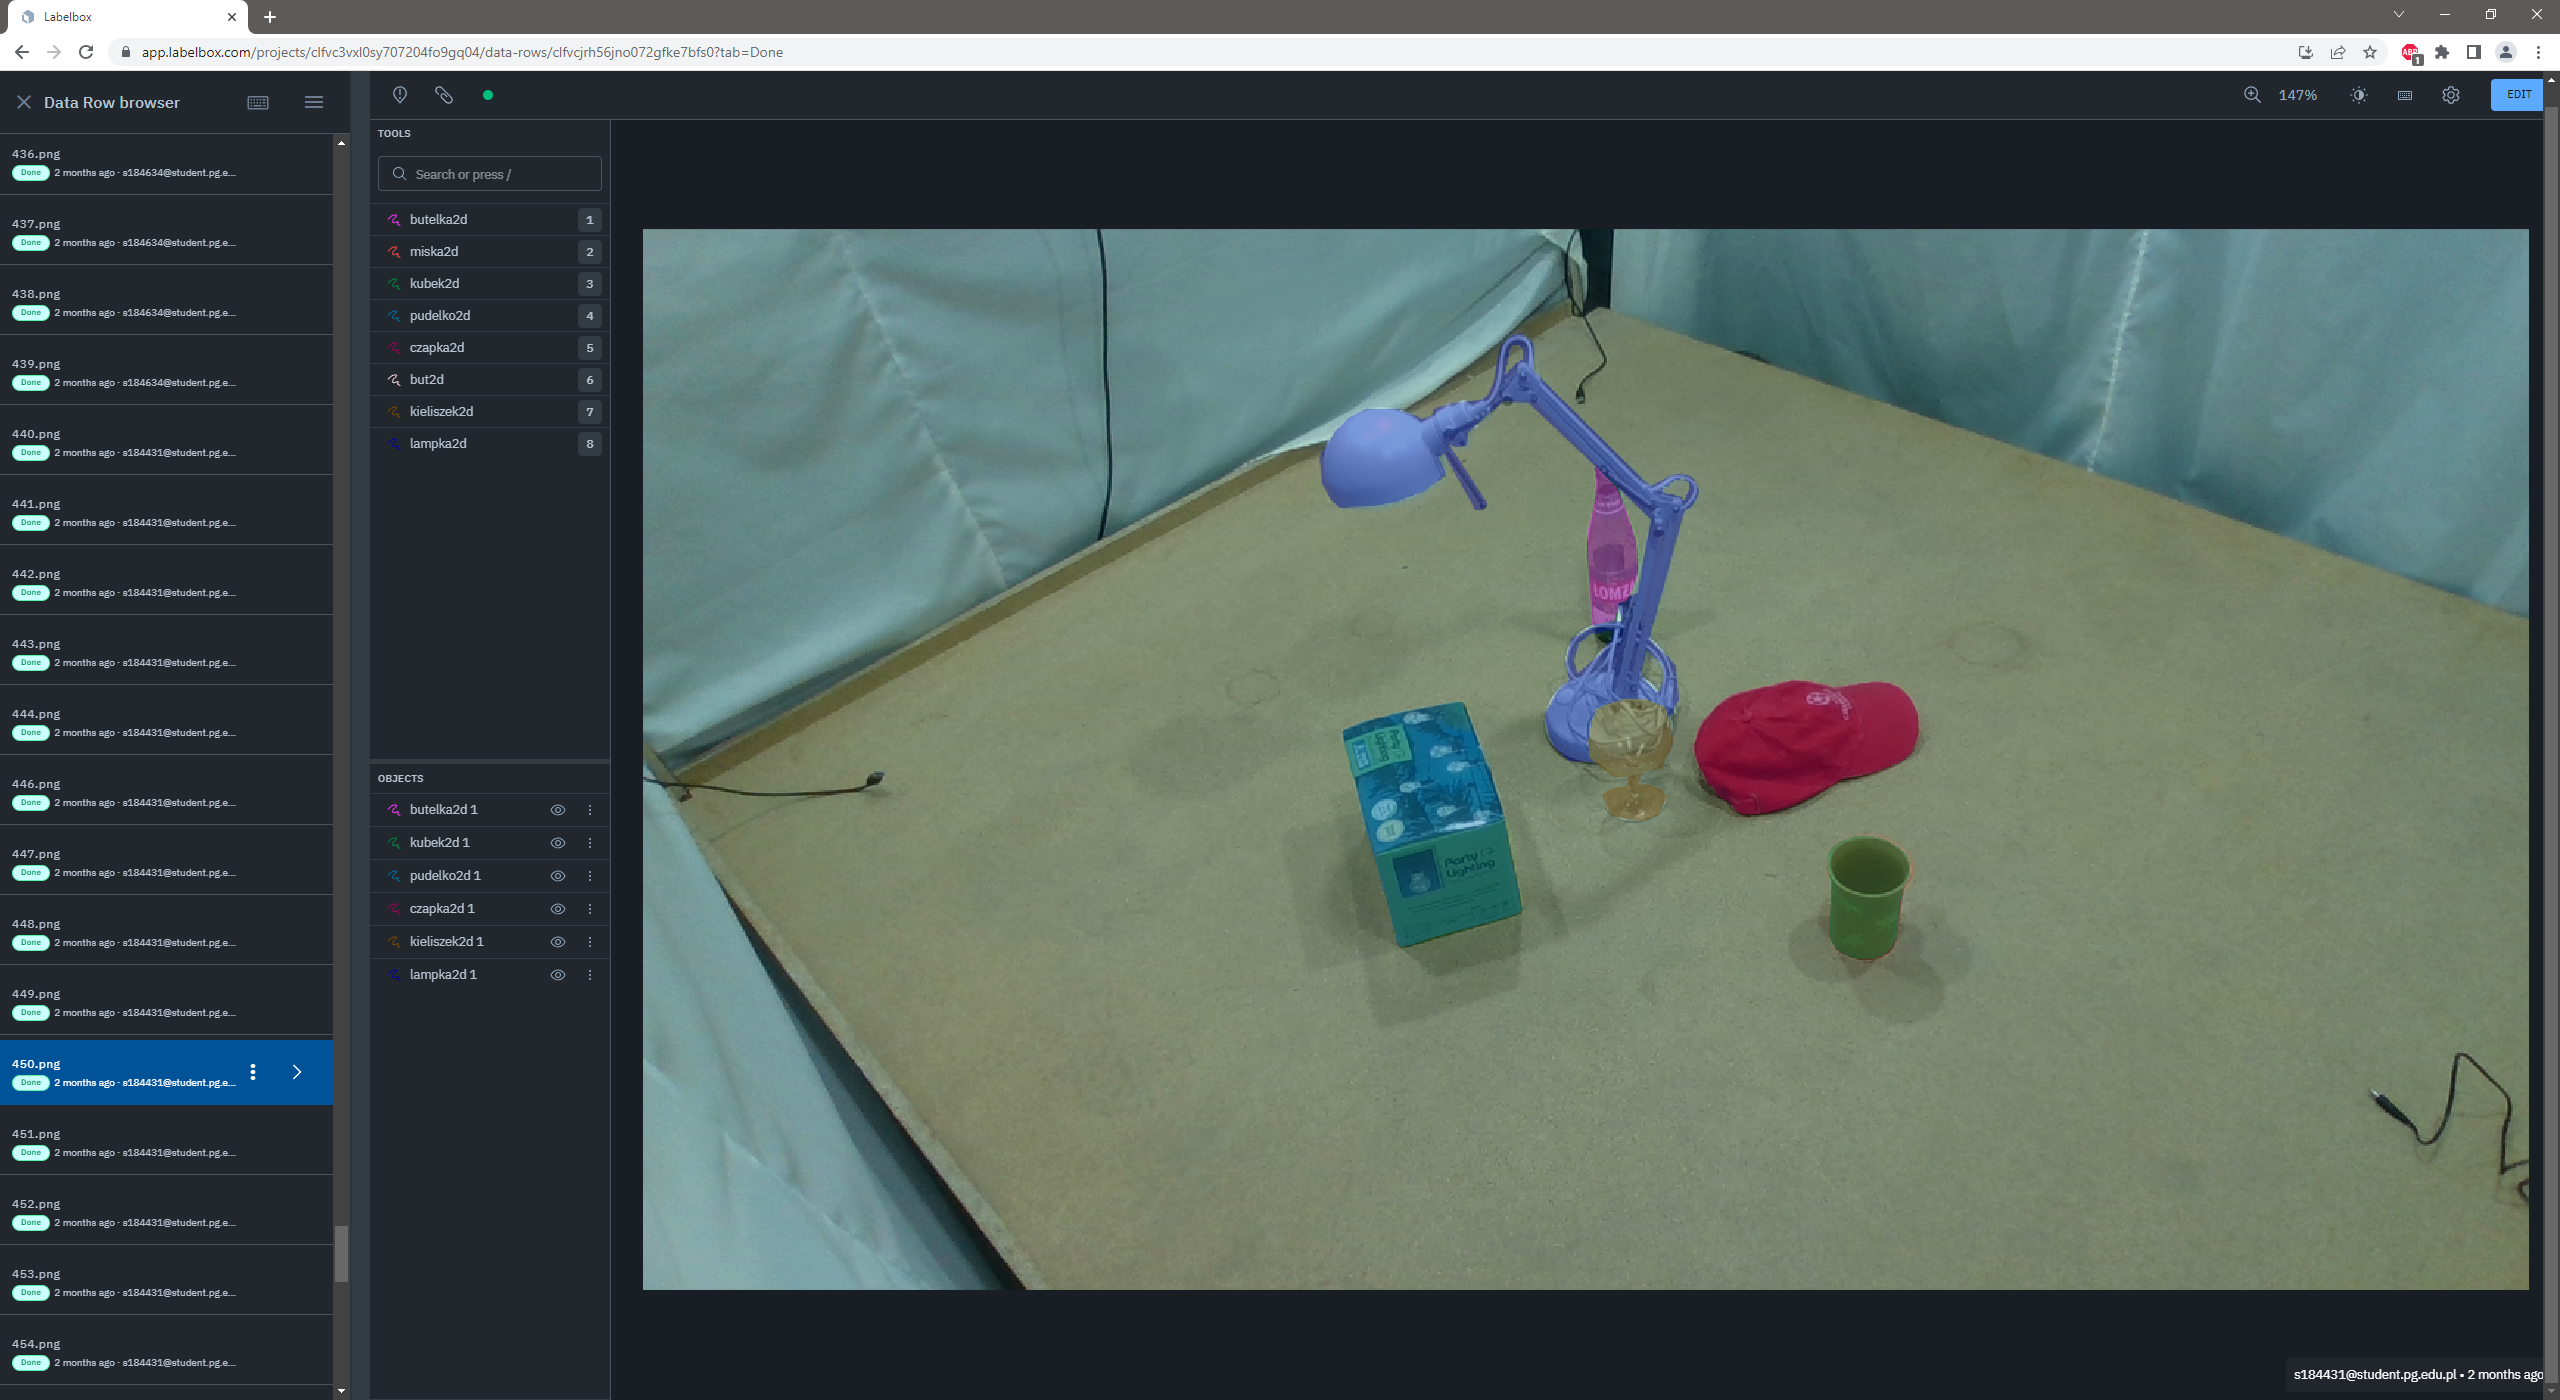
\includegraphics[width=0.8\textwidth]{img/labelbox-screenshot.png}
    \caption{One of the images from the dataset annotated in labelbox.}
    \label{fig:labelbox-window}
\end{figure}

Annotating, reviewing and reworking the images took 52 hours in total and was on of the most time-consuming tasks our team had to deal with.

\section{Segmentation algorithm}
Our Instance

\subsection{MaskRCNN for object segmentation in 2D}
We decided to use Mask R-CNN because it is a state-of-the-art Deep Convolutional Neural Network regarding image segmentation \cite{he2018mask, matterport_maskrcnn_2017}. This Neural Network detects objects in an image and generates a high-quality segmentation mask for each instance. It provides the vector of three essential factors for each object: instance mask, bounding box and label. Each of those elements is used in the following stages of image analysis (\cref{fig:app-flowchart}).

In our solution, the network got fine-tuned \cite{shinya2019understanding} on the dataset we made. The version used is Mask R-CNN v2 with a ResNet-50-FPN backbone \cite{li2021benchmarking}.

\subsection{Integration with the RGBD cameras}
We used the pyrealsense2 \cite{pyrealsense2-doc} library to get aligned RGB and depth frames from the cameras, and also to filter the depth image with temporal and spatial filtering. The RGB image is used as the input to MaskRCNN and the output masks are applied to the filtered depth image. This allows us to retrieve separate depth images of all the detected objects in the scene. These images are then used to create separate point clouds and draw bounding boxes around them using Open3D \cite{Zhou2018open3d}. The bounding boxes’ coordinates are extracted and used to project them onto the original RGB image.

\subsection{3D bounding boxes}
After familiarising ourselves with the concept of 3D bounding boxes (\textit{3DBB}) and the already existing methods of determining their placements \cite{MousavianAFK16}, we have devised our own 3DBB creating method relying on the functionalities of Open3D python library \cite{Zhou2018open3d} and processing of the point cloud. The first stage consists of extracting a part of the point cloud with our analysed object, based on its mask (\cref{fig:3dbb-mask}). To do that, we use Open3D, creating the object's bounding box (\cref{fig:pcloud-cutout}).

\begin{figure}[ht]
    \centering
    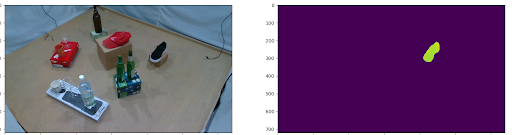
\includegraphics[width=0.8\textwidth]{img/mask.png}
    \caption{An example showing the RGB image and the mask of an object.}
    \label{fig:3dbb-mask}
\end{figure}

\begin{figure}[ht]
    \centering
    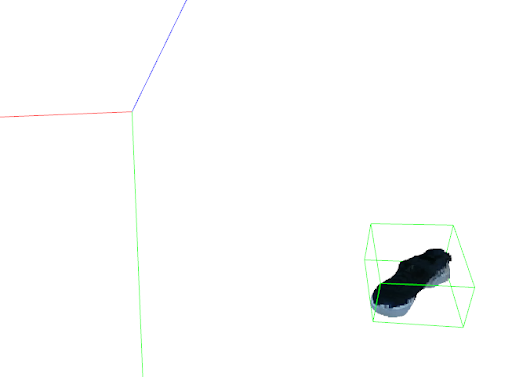
\includegraphics[width=0.4\textwidth]{img/pcloud-cutout.png}
    \caption{Fragment of the point cloud containing the previously shown object, with RGB image applied and a visible bounding box.}
    \label{fig:pcloud-cutout}
\end{figure}

After that, by getting the positions of 3DBB's vertices in the 3D space, the vertices' coordinates are transformed and properly placed on the 2D image using the OpenCV python library \cite{opencv_library}. The points are then connected by lines, comprising a 3D bounding box projected onto a two-dimensional plane (\cref{fig:pbbox-example}.

\begin{figure}[ht]
    \centering
    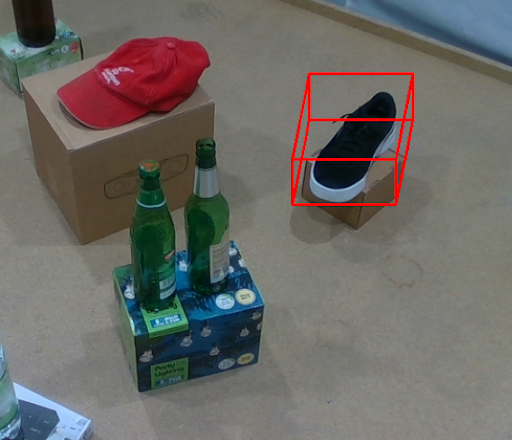
\includegraphics[width=0.4\textwidth]{img/bbox-example.png}
    \caption{A fragment of an RGB image showing the projected bounding box for an object.}
    \label{fig:pbbox-example}
\end{figure}

A key piece of information used while projecting the 3DBBs is the depth data, which has to be taken into account with the loss of the \textit{Z} dimension. It also allows us to determine the proportions of the boxes' edges to one another, which aids in the inspection of the projected points and automatic correction of their locations if any errors are found. The position of the 3DBB is checked in relation to the position of the object's mask, and in case of too big of a deviation, the bounding box's dimensions are corrected. 

Overall, we introduced a significant amount of parameters, which values were determined by trial and error, as well as variables which helped us control the correctness of the final coordinates of points on the 2D plane to properly replicate a 3D bounding box in a known environment and under known conditions. Of course, our approach is not perfect, and there are more accurate methods in existence. However, it does allow us to reconstruct an object's bounding box to a sufficient degree without using neural networks.


\chapter{Tests}
We discussed training 3D object detection models using proprietary datasets in the previous chapters. Once the models have been trained, the next crucial step is testing their performance and evaluating their effectiveness. This chapter will explore the various aspects of testing 3D object detection models trained on proprietary datasets.

We need a representative test dataset to evaluate the performance of our trained models. This dataset should ideally cover various scenarios, including different environmental conditions, object types, and object orientations. When using a proprietary dataset, ensuring that the test dataset is distinct and independent from the training data is essential to provide an unbiased evaluation.

To achieve this, we can separate the proprietary dataset into three subsets: the training, validation and test sets. We used the commonly used  proportions of 70 to 15 to 15 percentages. The training and validation sets are used exclusively during the training phase, while the test set is reserved for evaluating the model's performance. It is essential to ensure no overlap between the two sets to maintain the integrity of the evaluation.

\section{Evaluation Metrics}
We need suitable evaluation metrics to assess the performance of 3D object detection models. These metrics assess the accuracy and robustness of the model's predictions. 

\noindent We used the following metrics for 3D object detection:

\begin{itemize}
    \item \textbf{Intersection over Union (IoU):} IoU measures the overlap between the predicted and ground truth bounding boxes. It is computed by dividing the intersection volume by the union volume between the two boxes. This metric got used for three instances: 2D bounding boxes, instance masks and 3D bounding boxes.
    \item \textbf{Mean Average Precision (mAP):} mAP is the Average Precision value across different object classes. It provides an overall assessment of the model's performance in multiple categories.
    \item \textbf{Frames per second (FPS):} the frame rate at which consecutive images (frames) are captured or displayed. This metric is not typical for 3D object detection models, but in robotic environments or autonomous vehicles, the model’s speed is crucial. Obtained performance depends on many factors, like the number of objects in the scene and, most importantly, the camera's resolution. Because of that, in the summary of the model’s performance, we provided the results for two resolutions. 
\end{itemize}

\section{Testing Procedure}
To conduct the testing process, we feed the test dataset into the trained 2D object detection model and evaluate its predictions against the ground truth annotations. The following steps outline the testing procedure:

\begin{enumerate}
    \item \textbf{Input Preprocessing:} Similar to the training phase, the test dataset requires preprocessing. This involves transforming images and masks' associated annotations into a suitable format compatible with the model's input requirements.
    \item \textbf{Model Inference:} The preprocessed test data is passed through the instance segmentation model, which generates predictions for object classification and localisation. Our model defines localisation by two parameters: bounding box and mask.
    \item \textbf{Post-processing:} The raw predictions from the model often require post-processing steps to refine and filter the results. This may involve non-maximum suppression to remove redundant bounding boxes or score thresholding to filter out low-confidence predictions.
    \item \textbf{Evaluation:} Once the post-processing is complete, we compare the predicted bounding boxes, masks and labels with the ground truth annotations. We compute the evaluation metrics discussed earlier, including IoU and mAP to assess the model's performance on the test dataset.
\end{enumerate}

\section{Final statistics}
The final performance of the solution is: 
\begin{enumerate}[noitemsep]
    \item Intersection over union 2D: 81.3\%
    \item Intersection over union 3D: 80.9\%
    \item Mean average precision: 89.8\%
    \item Frame rate: 
    \begin{enumerate}[noitemsep, topsep=0pt]
        \item[-] 4 - 6 FPS for 1280x720 resolution 
        \item[-] 10 - 14 FPS for 640x360 resolution
    \end{enumerate}
\end{enumerate}
\chapter{Summary}
This project presents a novel proprietary 3D object detection model that demonstrates exceptional performance in terms of accuracy and efficiency. We introduce a cutting-edge model to address existing approaches' limitations and advance 3D object detection. Modern 3D detection models are based on advanced deep convolution neural networks. Our architecture is a hybrid approach using both analytical algorithms and neural networks.

Documentation begins with an overview of state-of-the-art solutions. It shows many different approaches to 3D object detection and emphasises the need for improved accuracy in detecting objects in three-dimensional space while ensuring real-time processing capabilities.

The proprietary model utilises innovative deep learning architectures and optimised algorithms. We describe the unique architectural design, which incorporates convolutional neural networks and analytical algorithms to get performance as good as possible regarding frame rate and accuracy. 

The \textit{Instance Segmentation} project was a valuable learning experience for the entire team. While working on it, we had to face different problems, both of technical and personal nature. We had to deal with problems concerning changes in the team members, both in the beginning and middle of the project and with the lab equipment not working properly.

Despite the project team's hardship during its development, we are satisfied with the results. Ultimately, we delivered a working program that fulfils all initial assumptions and leaves room for further development. While we are content, we realise some aspects of our program could be improved. We would be glad to work on these improvements in the future.

\chapter{Further development possibilities}
While working on the project, we tried to implement some solutions that did not work out in the end, mainly due to the lack of time. However, those failed attempts gave us ideas about the possible changes and improvements we could make in the future to make our program more accurate.

\section{Multiple RGBD cameras}
Attempts were made to integrate two RealSense cameras to get the same image from different angles, providing a more accurate point cloud. We did not succeed due to the problems with camera calibration, however if we were to continue the project, we would probably reattempt to do that with up to four cameras. Getting the depth data from four different angles would provide us with a very detailed point cloud with very few blind spots and an almost complete 3D reconstruction of the captured scenery, which would produce more accurate results for the 3DBB algorithm.

\section{Neural network for 3DBB estimation}
While we did experiment with different neural network models, in the end, we decided to go with an analytic approach, mostly due to the fact that a lot of models were outdated or required older versions of software and libraries which were very hard to acquire. There is a chance using a neural network to produce bounding boxes for objects would have given us more accurate results, however due to time constraints, we were forced to abandon the idea. We do, however, plan to try to run models again by setting up virtual machines with the required versions of the operating systems, libraries, software etc.

\section{Expanding the range of detectable objects}
The dataset which we worked on was supposed to consist of 8 classes, but due to different issues, it ended up containing only 7. This is a really small number of classes compared to the datasets available on the web. As of now, our datasets consist of about 900 RGBD images and over 5000 annotations of these seven classes, but we do plan to acquire more data and introduce more classes in the future.


\chapter{Encountered problems and their solutions}
Working on any project does not come without any problems. Some of the ones we encountered, we managed to resolve, some we were able to omit. This chapter provides an overview of the issues we had to face.

\section{The 'bottle' class}
Initially, our dataset was supposed to consist of 8 classes, one of them being the \textit{bottle} class. Unfortunately we did not take into the account the fact that PVC bottles allow the light to pass through them. The depth data for bottles was inaccurate and it showed \textit{'floating particles'} in places where the light passed through the plastic surface. This has made it very hard for our program to detect and calculate bounding boxes for this class, hence why we were forced to exclude this class from our dataset. However, we do plan to add other classes to our dataset to expand it and we might look into ways of ignoring those floating fragments of the depth cloud while creating bounding boxes for semi-transparent objects.

\section{Multiple cameras calibration - poor cable quality}
Unfortunately, due to poor cable quality in the lab, some of the cameras were recognised by the software as connected by USB 2.1, and the others were shown to have a proper USB 3.2 connection. Since USB 2.1 provides worse image quality, it was an issue when trying to calibrate multiple cameras so that they could work together. While we didn't succeed in doing so thins semester, we will look into solving that problem in the future.

\section{Starting up neural network models}
While we tried to launch several different neural network models we found, we did not achieve complete success with any of them. With how quickly everything develops, lots of the models turned out to require older, outdated versions of various libraries and softawres, which we were not able to launch or acquire. While this problem remains unsolved for now, we plan to set up virtual machine environments and try to run these models again.



\nocite{*}
\bibliographystyle{IEEEtran}
\bibliography{refs}


\end{document}